\chapter{Chaos, changing adversaries and quantum capability}\label{ch:chaos}

Every few months a headline announces that quantum computers will soon break the encryption
that protects banks, governments and hospitals. A reader who follows these reports may reach
a firm conclusion about disclosure control. The methods in this book assume an adversary of a
certain strength. A quantum computer is an adversary of a different order: it can factor the
numbers on which public-key encryption rests, and it can search large spaces faster than any
classical machine. On this view the floors, rounding and audits of the earlier chapters were
calibrated against yesterday's computers, and they will become obsolete when the new machines
arrive. The remedy is to move to stronger encryption now, before the data are exposed. The view
has real support. Shor's algorithms factor integers and compute discrete logarithms in polynomial
time on a quantum computer \citep{shor1997}, and the public-key systems in wide use today rest on
the hardness of exactly those problems.

The first fact that breaks the belief comes from the Bank's own register. The adversary who
most threatens a loan-level credit file is an insider at a reporting lender, who knows the
exposure of every loan his bank has reported. Against him the likelihood attack of
Chapter~\ref{ch:credit} names the right loan in 0.772 of attempts at the smallest floor examined,
and still in 0.416 at the largest. That attack compares one number with a short list of published
numbers. It needs no computer worth the name, and it reads a file the Bank meant to be read.
Encryption, of any strength, protects data that should not be read. A release is data that should
be. What an adversary can learn from a release is limited by what the release shows and by what
the adversary already knows, and computing power changes that limit only for attacks whose
bottleneck was computation.

This chapter asks one question. When the adversary changes, through drift in the world it
observes or through a new kind of computer, what has to change in the way the Bank decides, and
which tool answers each part? The answer separates three tasks that are easily run together:
forecasting how a scenario will develop, stress testing a decision against changes in its inputs,
and operating the systems that hold the data securely.

\section{A memo about quantum computers}

The chair of the Bank's statistics release committee received a memo from the Bank's information
technology department. It summarised a vendor briefing on quantum computing and recommended that
every file released by the statistics department be encrypted with a quantum-resistant algorithm.
The chair forwarded it to Naledi with a short question: did the committee's past decisions still
hold?

Naledi's reply began with Pieter. Pieter is a credit analyst at one of the Bank's reporting
lenders, the insider of Chapter~\ref{ch:credit}. If the Bank released a loan-level file, he would
download it from the Bank's website, open it in a spreadsheet, and look for the rows whose
exposures matched loans in his own bank's ledger. Encrypting the file in transit would change
nothing in that scene, because Pieter would be an authorised reader. The file would be decrypted
for him, as for every user, before he ever looked at it.

\section{Three roles that must stay apart}

The extension that this part of the book draws on uses three bodies of mathematics, and it
assigns each one a separate role. A dynamic model, such as the transport model of
Chapter~\ref{ch:dynamics}, may be used to forecast how a population of targets will move. Tools
from the study of chaos measure how sensitive a forecast, or a decision built on it, is to small
changes in its inputs, and so serve stress testing. Post-quantum cryptography protects the
register, its communications and its signatures against a specified class of cryptanalytic
attack, and so serves secure operation. These roles answer different questions, and naming the
three together creates no guarantee. Each component has its own assumptions and its own tests.

The confusion the roles prevent is concrete. A forecast is not a stress test: a model that
predicts the most likely path says nothing about how the decision behaves on the unlikely ones. A
stress test is not a security control: knowing that a decision survives perturbed inputs says
nothing about whether the keys that sign the decision record are safe. And a security control is
not a disclosure guarantee, as the scene with Pieter shows. The remainder of the chapter takes the
roles in turn, starting with sensitivity.

\section{Finite-time growth and the tangent equation}\label{c21:sec-growth}

Suppose a scenario model has a state $z(t)$ that evolves by $\dot z=F(z)$. The state might hold the
share of loans active in each size class, an attacker's measurement error, or a correlation
between exposures. Two runs that start a small distance apart will diverge or converge, and the
rate at which they do so measures how far the model's forecast can be trusted. To first order, a
small difference $v$ between two runs obeys the tangent equation
\begin{equation}\label{c21:eq-tangent}
\dot v=J_F\big(z(t)\big)\,v,\qquad v(0)=v_0,
\end{equation}
where $J_F$ is the Jacobian of $F$. The finite-time growth rate along one trajectory is
\begin{equation}\label{c21:eq-growth}
\lambda_T(z_0,v_0)=\frac1T\log\frac{\|v(T)\|}{\|v_0\|}.
\end{equation}
A positive value shows that small differences grew over that interval, for that trajectory, that
starting perturbation and that norm. It does not prove that the system is chaotic, which is a
statement about infinite time. The estimate also depends on the scaling of the coordinates, the
time step and transients at the start, so each of these must be reported. Over long horizons the
tangent vector grows too large to store, and the engine renormalises it at fixed intervals and
adds up the logarithms of the growth, as in the standard method of \citet{benettin1980}.

A numerical method for \eqref{c21:eq-growth} should be checked on a system whose answer is known before
it is trusted on one whose answer is not. Linear systems supply the check.

\begin{proposition}[Growth rates of a linear system]\label{c21:prop-linear}
Let $\dot z=Az$ with $A$ a constant matrix that is diagonalisable with real eigenvalues
$\mu_1>\mu_2\ge\dots\ge\mu_d$ and eigenvectors $w_1,\dots,w_d$.
\begin{enumerate}
\item If $v_0$ is an eigenvector with eigenvalue $\mu$, then $\lambda_T(z_0,v_0)=\mu$ for every $T>0$ and every $z_0$.
\item If $v_0=\sum_ia_iw_i$ with $a_1\ne0$, then $\lambda_T(z_0,v_0)=\mu_1+O(1/T)$ as $T\to\infty$.
\end{enumerate}
\end{proposition}

The engine's check takes $A$ diagonal with entries $0.5$ and $-1$ and starts the tangent along the
first axis, so the true rate is $0.5$ by part 1. Over a horizon of 4 the estimate was $0.5$ to twelve
decimal places (the draft of this book reports thirteen; the repository's code gives
$0.499999999999836$). The check confirms the integration and the renormalisation. Because the
starting direction is already the growing one, it does not test part 2, the slower convergence of
a general starting direction towards the fastest-growing one; a second check with a general start
would cover that.

\citet{lorenz1963} gave the classical example of a deterministic system with strong sensitivity
to initial conditions:
\begin{equation}\label{c21:eq-lorenz}
\dot z_1=\sigma(z_2-z_1),\qquad\dot z_2=z_1(\rho-z_3)-z_2,\qquad\dot z_3=z_1z_2-\beta z_3,
\end{equation}
with the familiar values $\sigma=10$, $\rho=28$ and $\beta=8/3$. These are a benchmark, not fitted
financial parameters. The engine ran the system for ten time units from $(1,1,1)$ to leave the
transient behind, then estimated the growth rate over a horizon of 60 with a time step of $0.005$,
starting the tangent along each of the three axes in turn. The three estimates were $0.882$,
$0.893$ and $0.861$, and the repository's code reproduces all three. They are positive and close to
one another, as part 2 of Proposition~\ref{c21:prop-linear} leads one to expect once each starting
direction has turned towards the fastest-growing one. The spread of about $0.03$ between them is
the finite-time variation that the definition warns about, and a longer horizon or several
starting points would be needed to narrow it.

The Bank's use for this is limited and specific. Naledi's scenario models for the credit file
describe how loan activity, exposures and an attacker's knowledge change from one vintage to the
next, in the manner of Chapter~\ref{ch:change}. A growth rate computed on such a model tells her
how quickly two scenarios that start almost together will come apart. A chaotic benchmark such as
Lorenz is a stress generator: a bounded transform of its trajectory can drive a synthetic
scenario parameter through irregular changes. The labels in such a study still come from running
the actual attack under each scenario. A chaotic trajectory is never evidence of disclosure, and
nothing in this book claims that real disclosure processes are chaotic. Nor is the decaying shear
of Chapter~\ref{ch:dynamics} chaotic; it was chosen because its solution is known.

\section{The diagnostic horizon}

The chair's reply to Naledi's first note asked a practical question. If a scenario model can
drift away from the truth, for how long does a release decision based on it remain valid? The
growth rate suggests an answer, and the answer must be handled carefully.

Suppose the attack response $g$ of Chapter~\ref{ch:dynamics} changes by at most $L_g$ for each unit of
change in the state, and that two states which start $\epsilon_0$ apart are about $e^{\lambda T}\epsilon_0$ apart at
time $T$. Then the risks computed from them differ by about $L_ge^{\lambda T}\epsilon_0$. Setting this equal to an
allowed error $\delta>L_g\epsilon_0$ gives the diagnostic horizon
\begin{equation}\label{c21:eq-horizon}
T_{\rm diag}\approx\frac1\lambda\log\frac{\delta}{L_g\epsilon_0}.
\end{equation}
With the Lorenz rate of about $0.88$ and an allowed error one hundred times the initial error after
scaling by $L_g$, the horizon is a little over five time units ($\log100/0.88=5.2$). The logarithm
makes the horizon grow slowly with precision: measuring the initial state ten times more accurately
adds only $\log(10)/\lambda$ to it.

\begin{example}[How long a scenario can be trusted]\label{c21:ex-horizon}
Suppose Naledi's scenario model grows small differences at the Lorenz rate, $\lambda=0.88$ per unit of
time. The other inputs are illustrative. The attack response moves by at most $L_g=0.5$ per unit of
state, the state is known to within $\epsilon_0=0.002$, and the committee will tolerate an error of
$\delta=0.02$ in a risk figure. Then $L_g\epsilon_0=0.001$, the ratio $\delta/(L_g\epsilon_0)$ is 20, and \eqref{c21:eq-horizon} gives
$\log(20)/0.88=3.4$ units of time. Measuring the state ten times more finely, to $0.0002$, raises the
ratio to 200 and the horizon to $6.0$, an extra $\log(10)/0.88=2.6$ units for a tenfold gain in
precision. If the model's unit is a month, Naledi would plan to rerun the scenario study after three
months. That is a date for a review. It does not end the certificate.
\end{example}

Equation \eqref{c21:eq-horizon} is a diagnostic, and it is not an expiry rule for audit certificates. Three
things stand in the way of reading it as one. The constant $L_g$ is rarely known. The growth rate is
not constant along a trajectory, as the spread of the Lorenz estimates shows. And the decision is not
a smooth function of the state: a release either passes the rule or it does not, and the exponential
bound says nothing about when a discontinuous decision changes. The engine's function returns an
infinite horizon for a nonpositive rate, which says only that this diagnostic sets no limit. What it
can do is shorten the period over which a forecast is relied on, and prompt a reassessment when the
scenario has had time to drift. The audit's validity rests on the conditions of Chapter~\ref{ch:monitoring}: the
release has not changed and the declared adversary still describes the threat.

\section{Decisions are discontinuous: perturb the decision}

A release rule compares an upper bound with a tolerance, and its output jumps from withhold to
release as the bound crosses the line. Near the line, the smallest change in an input can reverse
the decision; far from it, large changes leave it alone. A smooth sensitivity measure averages over
both situations and so describes neither. Global sensitivity analysis, which divides the variance of
a model's output among its inputs \citep{sobol2001,saltelli2007}, is built for smooth outputs; a
decision that jumps needs a measure of its own. The extension measures the decision directly. Perturb
the inputs many times, recompute the decision each time, and report the share of perturbed runs in
which it changed, the flip rate.

For a single risk estimate $b$, a tolerance $\tau$ and Gaussian perturbations, the flip rate has a
closed form.

\begin{proposition}[Flip rate near a threshold]\label{c21:prop-flip}
Let the decision be $d(z)=\mathbf 1\{z>\tau\}$, let $b\ne\tau$, and let $Z\sim N(0,1)$. For $s>0$, the
probability that $d(b+sZ)\ne d(b)$ is $\Phi\big(-|\tau-b|/s\big)$, where $\Phi$ is the standard normal
distribution function.
\end{proposition}

The flip rate depends only on the distance to the tolerance measured in units of the perturbation.
Figure~\ref{c21:fig-flip} sets the formula beside the engine's simulation. With a tolerance of $0.12$, a perturbation
standard deviation of $0.01$ and 2,000 draws at each point, the repository's run with seed 2026 gave
flip rates of 0 at an estimate of $0.05$, $0.022$ at $0.10$, $0.298$ at $0.115$ and $0.454$ at $0.119$. The formula gives
$0.000$, $0.023$, $0.309$ and $0.460$. The draft reports $0.309$ and $0.470$ at the last two points, from a different
random stream; with 2,000 draws the standard error at these points is about $0.010$ to $0.011$, so
the simulated rates differ from the formula by at most about one standard error in every case.

\begin{example}[One estimate, two widths of doubt]\label{c21:ex-flip}
An upper bound of $0.110$ sits $0.010$ below the tolerance of $0.12$. If the inputs behind it are uncertain by a standard
deviation of $0.01$ in their effect on the bound, the distance is one width, and
Proposition~\ref{c21:prop-flip} gives a flip rate of $\Phi(-1)=0.159$. The engine, perturbing the bound 2,000 times with
seed 2026, counted 290 flips, a rate of $0.145$, within one standard error ($0.008$) of the formula. If the uncertainty doubles to $0.02$, the distance is
half a width and the formula gives $\Phi(-0.5)=0.309$; the engine counted 595 flips, $0.298$, again within
one standard error. (The draft prints 293 and 624 from its own random stream.) The bound did not move. Only the committee's doubt about
its inputs did, and that alone doubled the share of nearby worlds in which the decision would go the
other way.
\end{example}

\begin{figure}[ht]
\centering
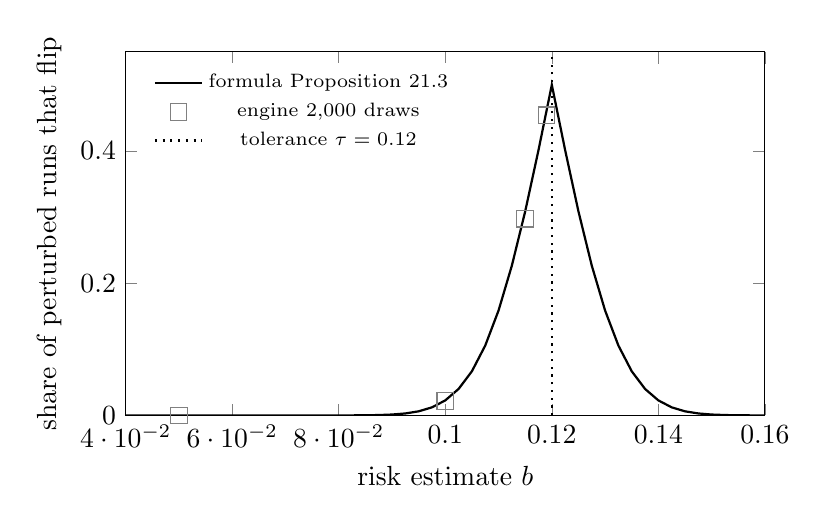
\begin{tikzpicture}
\begin{axis}[width=0.8\textwidth,height=6.2cm,xlabel={risk estimate $b$},ylabel={share of perturbed runs that flip},
  xmin=0.04,xmax=0.16,ymin=0,ymax=0.55,
  legend style={at={(0.03,0.97)},anchor=north west,draw=none,font=\scriptsize,fill=white}]
\addplot[black,thick] coordinates {(0.0400,0.00000) (0.0425,0.00000) (0.0450,0.00000) (0.0475,0.00000) (0.0500,0.00000) (0.0525,0.00000) (0.0550,0.00000) (0.0575,0.00000) (0.0600,0.00000) (0.0625,0.00000) (0.0650,0.00000) (0.0675,0.00000) (0.0700,0.00000) (0.0725,0.00000) (0.0750,0.00000) (0.0775,0.00001) (0.0800,0.00003) (0.0825,0.00009) (0.0850,0.00023) (0.0875,0.00058) (0.0900,0.00135) (0.0925,0.00298) (0.0950,0.00621) (0.0975,0.01222) (0.1000,0.02275) (0.1025,0.04006) (0.1050,0.06681) (0.1075,0.10565) (0.1100,0.15866) (0.1125,0.22663) (0.1150,0.30854) (0.1175,0.40129) (0.1200,0.50000) (0.1225,0.40129) (0.1250,0.30854) (0.1275,0.22663) (0.1300,0.15866) (0.1325,0.10565) (0.1350,0.06681) (0.1375,0.04006) (0.1400,0.02275) (0.1425,0.01222) (0.1450,0.00621) (0.1475,0.00298) (0.1500,0.00135) (0.1525,0.00058) (0.1550,0.00023) (0.1575,0.00009) (0.1600,0.00003)};
\addplot[gray,only marks,mark=square,mark size=3pt] coordinates {(0.05,0) (0.10,0.022) (0.115,0.2975) (0.119,0.454)};
\addplot[dotted,thick] coordinates {(0.12,0) (0.12,0.55)};
\legend{formula Proposition 21.3,engine 2{,}000 draws,tolerance $\tau=0.12$}
\end{axis}
\end{tikzpicture}
% source: recomputed with privacy_risk.sensitivity.decision_flip_rate, seed 2026
\caption{Flip rate of a threshold decision against the risk estimate, with Gaussian perturbations of
standard deviation $0.01$ and tolerance $0.12$. The formula of Proposition~\ref{c21:prop-flip} (solid black line)
is set beside the engine's simulated rates (open grey squares); the dotted line marks the tolerance.
Synthetic study.}
\label{c21:fig-flip}
\end{figure}

The figure carries the lesson of the section. An estimate of $0.10$, which a committee would read as
comfortably inside a tolerance of $0.12$, flips in about one perturbed run in fifty. An estimate of
$0.115$ flips in almost one in three. A model that forecasts risk well on average can be unsafe for
exactly the decisions near the line, and those are the ones a committee most needs to get right.
Stress effort belongs there: on configurations close to the tolerance and on cases where the ranking
of candidate settings reverses.

In practice the perturbed quantities are the inputs of the attack: the attacker's measurement
error, correlations between exposures, which loans are active, when the release happens and what
the attacker knows. The decision to perturb is the one the release rule makes, recomputed with the
attack run again under each perturbed input. For Pieter the input that moves is the precision of
his reading. A lender that improves its ledger, or a merger that brings a second lender's ledger
into his hands, changes the adversary without changing the release. The flip rate shows how close
the committee's decision sits to the point where such a change would reverse it.

\section{A stress gate over a preregistered set}

A flip rate describes the decision. To act on it, the release rule itself must take account of the
stress scenarios. Let $\mathcal S$ be a finite set of stress scenarios, written down before any audit is
run, and let $R_{a,s}(\theta)$ be an upper confidence bound on the success of attack $a$ under scenario $s$
for protection setting $\theta$. The gate releases $\theta$ only if
\begin{equation}\label{c21:eq-gate}
\max_{s\in\mathcal S}R_{a,s}(\theta)\le\tau_a\qquad\text{for every required attack }a.
\end{equation}
The engine calls this a robust gate. Its guarantee is exactly as wide as the set.

\begin{proposition}[Coverage of the stress gate]\label{c21:prop-gate}
Let the bounds $R_{a,s}(\theta)$ be simultaneous at level $1-\alpha$ over every candidate setting $\theta$,
required attack $a$ and scenario $s\in\mathcal S$: with probability at least $1-\alpha$,
$r_{a,s}(\theta)\le R_{a,s}(\theta)$ for all of them at once. Then with probability at least $1-\alpha$, every setting
that passes \eqref{c21:eq-gate} has true risk at most $\tau_a$ for every required attack and every scenario in $\mathcal S$,
whatever setting is chosen among those that pass.
\end{proposition}

The proposition needs the error allocation to cover every coordinate the gate looks at. Adding
scenarios to $\mathcal S$ therefore costs audit budget, in the way that adding candidate settings did in
Chapter~\ref{ch:selection}. It says nothing about scenarios outside the set. A finite grid of stress scenarios does not
bound a continuum of them unless a separate argument, a covering or a regularity condition, is
supplied. And a scenario with no bound counts as a failure: the gate cannot pass an attack it has
not audited.

The evidence run illustrates the last point with the credit-register figures of the earlier
chapters, through the release gate of Chapter~\ref{ch:learning}. With the pooled history attack and the insider
both required at a tolerance of $0.12$, the gate withheld the file: at a floor of 75 the insider had
not been audited, and at a floor of 150 its bound of $0.42$ failed. With only the outside attack
required, the gate released at a floor of 75. The choice of which adversaries are required is a
declaration the committee makes, as Chapter~\ref{ch:scenario} insists, and the gate makes the consequence of that
declaration visible.

\begin{example}[Three stress scenarios for one attack]\label{c21:ex-gate}
Take the floor of 75 and the external attack at a tolerance of $0.12$, with three preregistered
scenarios: the base case with a bound of $0.104$, a case in which the adversary's readings are twice
as precise with a bound of $0.112$, and a case in which a lender merger gives the adversary a second
ledger, with a bound of $0.131$. The base bound is the run's figure; the other two are illustrative.
The stress gate takes the worst scenario, $0.131$, and fails the floor, naming the merger as the
reason. Drop the merger from the set and the gate passes, because its guarantee covers only the set.
Add the insider as a required attack with no audit and the gate fails again, on the missing
coordinate. Each scenario also costs attacks: with two candidates and three scenarios the $0.05$ is
split six ways, and the zero-success audit at $0.12$ needs 38 attacks per coordinate instead of 24
($\lceil\log(0.05/6)/\log(0.88)\rceil=38$ against $\lceil\log(0.05)/\log(0.88)\rceil=24$).
\end{example}

Naledi's draft reply to the chair now had two parts. The first explained that the committee's
decisions depended on which adversaries it declared, and that the insider row, Pieter's row, was
the one that withheld the loan-level file. The second part was about the memo, and for that she
needed to separate what a quantum computer could do to the Bank's systems from what it could do
with the Bank's releases.

\section{What quantum capability changes}

A quantum threat model has to say what algorithm the attacker runs, how the input is represented,
what access the attacker has to the system under attack, what resources the attack needs and what
counts as success. Two algorithms anchor most discussion. Shor's algorithms factor integers and
compute discrete logarithms in polynomial time \citep{shor1997}, which breaks the public-key systems
based on those problems once a large enough fault-tolerant machine exists. Grover's algorithm
searches an unstructured space of $N$ items in about $\sqrt N$ queries to an oracle, where a classical
search needs about $N$ \citep{grover1996}. The first is a large speed-up on a narrow class of
problems. The second is a modest speed-up on a broad one, and it assumes an oracle that can be built
and run coherently. Neither result says that a quantum computer can identify every record in a
database or solve every learning problem. Loading data, building a reversible oracle, correcting
errors and repeating measurements all bear on what a concrete attack would cost.

Figure~\ref{c21:fig-threats} separates the two threats that the memo had merged. The first is an attack on the
cryptography that protects the register, the channels that carry its data, the keys and the
signatures on decision records. Shor's algorithms are the reason this threat is real, and an
adversary may record encrypted traffic today in the hope of decrypting it later. The second is an
attack that uses stronger computation to infer identities or attributes from an authorised or
public release. These threats call for different defences, run by different parts of an
institution. Stronger encryption does not remove information that a release shows to its readers,
and a good disclosure audit does not protect a weak transport protocol or a stolen signing key.

\begin{figure}[ht]
\centering
\begin{tikzpicture}[>=stealth,node distance=0.6cm,
  box/.style={draw,minimum width=3.6cm,minimum height=1.2cm,align=center,font=\small}]
\node[box,pattern=north east lines,pattern color=gray!60] (a1) at (0,1.8) {};
\node[box,fill=white,minimum width=3.2cm,minimum height=0.9cm] at (0,1.8) {register, channels,\\ keys, signatures};
\node[box,fill=white] (b1) at (5,1.8) {cryptanalysis\\ (Shor)};
\node[box,fill=white] (c1) at (10,1.8) {post-quantum standards;\\ security programme};
\node[box,fill=gray!25] (a2) at (0,0) {released file,\\ read by its users};
\node[box,fill=gray!25] (b2) at (5,0) {inference from\\ what is shown};
\node[box,fill=gray!25] (c2) at (10,0) {attack audits;\\ formal privacy};
\draw[->,thick] (a1)--(b1); \draw[->,thick] (b1)--(c1);
\draw[->,thick,dashed] (a2)--(b2); \draw[->,thick,dashed] (b2)--(c2);
\node[font=\scriptsize] at (0,2.75) {what is attacked};
\node[font=\scriptsize] at (5,2.75) {threat};
\node[font=\scriptsize] at (10,2.75) {defence};
\end{tikzpicture}
\caption{Two threats from a quantum-capable adversary and their separate defences. The upper row
(hatched box, solid arrows) is the attack on cryptography, answered by the security programme. The
lower row (grey box, dashed arrows) is inference from a release, answered by attack audits and, where it
applies, formal privacy. Each row's defence does nothing against the other row's threat.}
\label{c21:fig-threats}
\end{figure}

For the second threat, the useful question is whether the attack was ever limited by computation.
Some attacks are. The reconstruction of census microdata from published tables solved a very large
system of constraints, and computing power was part of what made it possible
\citep{garfinkel2019,abowd2022}. A faster solver could reach further along that road. Other attacks
are limited by information. A linkage attack against a cell of a few hundred loans compares a
reading with a few hundred numbers, and no speed-up is needed. What stops it, when anything does,
is that the release does not distinguish the target from the other candidates. No amount of
computation changes that.

\begin{proposition}[Computation cannot separate what the release does not]\label{c21:prop-info}
Let the target be one of the candidates in a released file, and let $Z$ be everything the adversary
holds: the release and its own auxiliary information. Suppose that, given $Z$, the target is equally
likely to be each of $r\ge1$ candidates and has probability zero of being any other. Let $d(Z,U)$ be any
procedure that names a candidate, where $U$ is randomness independent of the target given $Z$. Then
$\Prob\{d(Z,U)=\text{target}\}\le1/r$.
\end{proposition}

The procedure $d$ is unrestricted. It may run for any length of time, and it may be a quantum
computation that starts from a fixed state, takes $Z$ as classical input and is measured at the end,
because the outcome of such a computation is a random function of $Z$ with randomness that does not
depend on which candidate is the target. The bound is the plain maximum of the posterior from
Chapter~\ref{ch:scenario}, and it applies to every attack at once. Chapter~\ref{ch:credit} gave the same ceiling of $1/r$
for Pieter's likelihood attack when $r$ candidates publish his target's value; the present result says
that a cleverer attack, run on a stronger computer, could not do better. The condition is about
information. If the adversary gains new information, $Z$ changes and the ceiling may rise. A
stronger computer gives no new information.

The same reasoning shows the limit of the proposition. When the posterior is not flat, when the
release does separate the target, a classical attack that fails to find the most probable
candidate leaves room that a stronger computer might fill. The audits in this book measure the
attacks they implement, and a classical red-team exercise cannot certify all quantum attacks by
giving them a larger budget label. A quantum attack study needs an implemented attack or a
defensible resource analysis. Until one exists, the engine records quantum attack coverage on
released data as unresolved, neither zero nor covered.

The chair read this section of Naledi's note twice. Her question at the committee was whether the
Bank could say that its releases were safe against quantum computers. Naledi said the Bank could
say three narrower things: that its released files were audited against the attacks it had
declared, that for files where the target cannot be separated from others no computer could do
better than chance among them, and that quantum attacks on releases were recorded as not yet
studied. The committee minuted all three.

\section{Post-quantum standards belong in the security programme}

The memo's recommendation was not wrong about the first threat. The register, the channels that
carry supervisory data to the Bank and the signatures on its records do rest on public-key systems
that a large quantum computer could break. The answer to that threat is published. NIST has
standardised ML-KEM for establishing keys \citep{nist2024a}, and ML-DSA and SLH-DSA for digital
signatures \citep{nist2024b,nist2024c}. These are designed to resist quantum cryptanalysis under
their stated assumptions. They do not guarantee security against every future discovery or against
a faulty implementation.

The standards are components, and their use has conditions. ML-KEM establishes shared key
material; it does not by itself encrypt bulk data, and it must sit inside an authenticated
protocol with key derivation, authenticated encryption and key management. A signature shows that a
record came from the holder of a key and has not changed since. It does not show that the counts in
the record are true or that the operator followed the audit procedure. The trust and independence
requirements on the audit registry, set out in Chapter~\ref{ch:learning}, stay in force whatever signature
scheme is used.

The engine follows a simple division of labour. It contains no cryptography of its own. Its
decision records carry SHA-256 digests, which detect change but say nothing about who made a
record; signing records, and protecting the register and its transport against quantum-capable
attackers, belong to the institution's security programme, using maintained implementations of the
three standards through supported protocols. The engine's documentation also forbids two tempting
shortcuts. It forbids bespoke ciphers, including the chaotic ciphers that a reader of the earlier
sections might be drawn to and that cryptographers have found weak in many published designs
\citep{alvarez2006}, and it forbids deriving keys or randomness from model trajectories. A Lorenz
trajectory is unpredictable in the sense of Section~\ref{c21:sec-growth}: small errors in its start grow fast. It
is fully determined by that start, and an adversary who learns the start and the parameters can
reproduce it exactly. Numerical unpredictability is not cryptographic entropy.

The security work the memo called for is therefore real, and it has a sequence: list the
public-key dependencies, establish how long each kind of data must stay confidential and compare
that with the time a migration will take \citep{mosca2018}, identify stored ciphertext that must
survive future cryptanalysis, choose maintained implementations through the security process, and
test interoperability and downgrade behaviour. The chair sent the memo back to the information
technology department with a request for that plan, and a note that encrypting released files was
not part of it.

\section{A guarantee that does not depend on the attacker's computer}

There is one disclosure guarantee in this book that holds whatever computer the attacker uses.
Chapter~\ref{ch:dp} set out differential privacy: a randomised mechanism $M$ is $(\varepsilon,\delta)$-differentially private
when, for neighbouring datasets $D$ and $D'$ and every set $S$ of outputs,
\begin{equation}\label{c21:eq-dp}
\Prob\{M(D)\in S\}\le e^{\varepsilon}\,\Prob\{M(D')\in S\}+\delta.
\end{equation}
The guarantee is a property of the mechanism's output distributions, so it does not depend on the
attacker's running time \citep{dwork2014}. What it does not say directly is how it applies when
the classical output is fed into a quantum computation. The extension supplies the step for one
restricted setting.

\begin{proposition}[Postprocessing by a data-independent quantum computation]\label{c21:prop-post}
Let $M$ satisfy \eqref{c21:eq-dp}. Let a later computation take the classical output $y$ of $M$, start from a fixed
state that does not depend on the dataset, and end in an event $B$ with probability $h_B(y)\in[0,1]$.
Then
\begin{equation}\label{c21:eq-post}
\E\,h_B\big(M(D)\big)\le e^{\varepsilon}\,\E\,h_B\big(M(D')\big)+\delta.
\end{equation}
\end{proposition}

The left side is the probability that the whole procedure, mechanism followed by quantum
computation, ends in $B$ when the data are $D$, and the right side bounds it in terms of the same
procedure on $D'$. So the classical guarantee carries over, with the same parameters, to anything
such a computation does with the output. The proof applies \eqref{c21:eq-dp} to the sets on which $h_B$ exceeds
each level and integrates over the levels.

The engine checks the inequality numerically. For randomised response with $\varepsilon=\log3$, which
reports a respondent's true bit with probability $3/4$, the output distributions on neighbouring
datasets are $(0.75,0.25)$ and $(0.25,0.75)$. Figure~\ref{c21:fig-post} shows the two sides of \eqref{c21:eq-post} for three
choices of $h_B$. When $h_B$ is the indicator of the first output, the left side is $0.75$ and the right
side is $3\times0.25=0.75$, so the inequality holds with equality: this is the privacy condition itself
on its tightest set. For $h_B=(0.3,0.9)$ the sides are $0.45$ and $2.25$, and for the constant
$h_B=(0.6,0.6)$ they are $0.60$ and $1.80$.

\begin{figure}[ht]
\centering
\begin{tikzpicture}
\begin{axis}[ybar,width=0.8\textwidth,height=6cm,bar width=16pt,ymin=0,ymax=2.6,ylabel={value},
  symbolic x coords={{$h_B=(1,0)$},{$h_B=(0.3,0.9)$},{$h_B=(0.6,0.6)$}},xtick=data,enlarge x limits=0.25,
  legend style={at={(0.03,0.97)},anchor=north west,draw=none,font=\scriptsize,fill=white}]
\addplot[fill=gray!25,postaction={pattern=north east lines,pattern color=gray!70}] coordinates {({$h_B=(1,0)$},0.75) ({$h_B=(0.3,0.9)$},0.45) ({$h_B=(0.6,0.6)$},0.60)};
\addplot[fill=black!70] coordinates {({$h_B=(1,0)$},0.75) ({$h_B=(0.3,0.9)$},2.25) ({$h_B=(0.6,0.6)$},1.80)};
\legend{left side $\E h_B(M(D))$,right side $e^{\varepsilon}\E h_B(M(D'))$}
\end{axis}
\end{tikzpicture}
% source: privacy_risk.dp.postprocessing_bound; tests/test_ext_sensitivity.py
\caption{The two sides of the postprocessing inequality \eqref{c21:eq-post} for randomised response with
$\varepsilon=\log3$ and three later computations $h_B$. Left sides are light and hatched; right sides are dark
and plain. The first pair is equal, the tight case; in the other two the bound holds with room.
Synthetic check.}
\label{c21:fig-post}
\end{figure}

The proposition has firm limits, and they should travel with it. It assumes the quantum
computation starts from a state that does not depend on the confidential data. If the attacker
holds quantum side information correlated with the dataset, or can query the private mechanism
coherently, the argument does not apply, and a guarantee for that setting needs its own definition
and proof. It is a statement about a distributional inequality, not a claim that any system defeats
a quantum computer. And everything Chapter~\ref{ch:dp} said about the meaning of $\varepsilon$ still holds: the
guarantee limits the change caused by one person's contribution, it does not hide population facts,
and against an adversary who arrives with a strong prior it can permit a high posterior. Repeated
releases need composition accounting, and any published model, selected setting or audit statistic
is an output that must be assessed too.

Pieter, at his desk at the lender, has an ordinary laptop. The committee's decision on the
loan-level file did not turn on what that laptop could compute. It turned on what the file would
show him, and that would be the same on any machine he could buy or rent.

\section{The answer}

The chapter asked what has to change in the way the Bank decides when the adversary changes, and
which tool answers each part. When the world the adversary observes drifts, the Bank should measure
how sensitive its decision is: by finite-time growth rates checked first on a system with a known
answer, by flip rates of the decision itself near the tolerance, and by a gate that requires every
preregistered stress scenario to pass under a simultaneous error allocation. The diagnostic
horizon prompts reassessment and does not replace it. When the adversary acquires a new kind of
computer, two separate things change. The cryptography that protects the register and its records
must move to the published post-quantum standards through the security programme, with no bespoke
or chaotic ciphers. The disclosure risk of a release changes only where an attack was limited by
computation; where the release cannot separate a target from its neighbours, no computation can,
and where it can, the Bank must record quantum attacks as unstudied until a study exists.
Differential privacy is the one guarantee whose strength does not depend on the attacker's
computer, and it carries over to data-independent quantum postprocessing. Quantum computers do not
make disclosure control obsolete, and stronger encryption does not replace it, because disclosure
control governs what the Bank chooses to show.

\begin{inpractice}[In practice: changing adversaries and new computers]
Declare the stress scenarios before the audit, allocate the error budget across every candidate,
attack and scenario, and treat a scenario with no bound as a failure. Report the flip rate of the
decision for configurations within a few perturbation widths of the tolerance. Use growth rates and
the diagnostic horizon to schedule reassessment, never as an expiry date. Keep two registers of
threat: send attacks on cryptography to the security programme, with a migration plan built on
FIPS 203, 204 and 205 and maintained implementations, and keep attacks on releases in the
disclosure record, with quantum attack coverage marked as unresolved until a study exists. Where a
release carries a differential privacy guarantee, state that it extends to data-independent
quantum postprocessing and does not extend to correlated quantum side information.

\medskip\noindent\textit{In the software.} Growth rates, the Lorenz benchmark, the diagnostic horizon, flip rates and the
stress gate are in \texttt{privacy\_risk.sensitivity} (\texttt{finite\_time\_growth}, \texttt{lorenz},
\texttt{diagnostic\_horizon}, \texttt{decision\_flip\_rate}, \texttt{robust\_gate}). The postprocessing check is
\texttt{privacy\_risk.dp.postprocessing\_bound}. The tests are in \texttt{tests/test\_ext\_sensitivity.py}: the growth rate on a linear system and then Lorenz, the flip rate with the stress gate, and the postprocessing inequality for randomised response. The cryptography policy is in \texttt{SECURITY.md}. Algorithm~21.1 gives the flip rate, which is a direct count, and Algorithm~21.2 the stress gate; their checks replay Examples~\ref{c21:ex-flip} and~\ref{c21:ex-gate}.
\end{inpractice}

\begin{mdframed}[linecolor=gray!60,backgroundcolor=gray!5]
\textbf{Algorithm 21.1.} Decision flip rate.\par\smallskip
\textit{Input.} A decision rule $d$; base inputs $b=(b_1,\dots,b_m)$; perturbation standard deviations
$s=(s_1,\dots,s_m)$; a number of draws $N$; a seeded random source.\par
\textit{Output.} The reference decision $d(b)$, the number of flips, $N$, and the flip rate.
\begin{enumerate}
\item Refuse the inputs unless $s$ has one entry for each input, every $s_i\ge0$, and $N\ge1$.
\item Compute the reference decision $d(b)$.
\item For each of $N$ draws, draw independent standard normal $Z_1,\dots,Z_m$, compute $d(b_1+s_1Z_1,\dots,b_m+s_mZ_m)$, and count a flip if it differs from $d(b)$.
\item Return the number of flips $F$ and the flip rate $F/N$. For one estimate and the rule $d(z)=\mathbf 1\{z>\tau\}$, the rate estimates $\Phi(-|\tau-b|/s)$ of Proposition~\ref{c21:prop-flip}.
\end{enumerate}
\textit{Checks (seed 2026, the repository's random stream; the draft's counts of 293 and 624 came from another):}
\begin{itemize}
\item An upper bound of $0.110$ against a tolerance of $0.12$, standard deviation $0.01$, 2,000 draws (Example~\ref{c21:ex-flip}), number of flips: 290.
\item The same with standard deviation $0.02$: 595.
\item The same, flip rate: 0.298 (to three places, $0.2975$).
\item A standard deviation of zero, flip rate: 0.000.
\item A negative standard deviation: refused.
\item Two standard deviations for one input: refused.
\end{itemize}

\medskip
\textbf{Algorithm 21.2.} The stress gate over a preregistered set.\par\smallskip
\textit{Input.} The required attacks $a$, each with a tolerance $\tau_a$; for each attack, the upper bounds
$R_{a,s}$ under the preregistered scenarios $s\in\mathcal S$, computed with an error allocation that covers every
candidate, attack and scenario.\par
\textit{Output.} Pass or fail, with each failure named by its attack and its worst scenario, or marked missing.
\begin{enumerate}
\item For each required attack $a$: if it has no bound under any scenario, record it as missing.
\item Otherwise find the scenario $s$ with the largest bound; if $R_{a,s}>\tau_a$, record $a$ as failed under $s$, with that bound.
\item Pass if and only if nothing was recorded, which is \eqref{c21:eq-gate}. The pass says nothing about scenarios outside $\mathcal S$ (Proposition~\ref{c21:prop-gate}).
\end{enumerate}
The gate checks no input beyond the presence of a tolerance, so its only refusal is an empty list of required attacks.\par
\textit{Checks:}
\begin{itemize}
\item The external attack at $0.12$ with base, precise-reading and merger scenarios at $0.104$, $0.112$ and $0.131$ (Example~\ref{c21:ex-gate}), scenario named in the failure: merger.
\item The same without the merger, number of failures: 0.
\item The same with the insider also required and no insider audit, reason for the failure: missing.
\end{itemize}
\end{mdframed}

\section{Proofs}

\begin{proof}[Proof of Proposition~\ref{c21:prop-linear}]
For a linear system the Jacobian is $A$ at every state, so the tangent equation \eqref{c21:eq-tangent} is
$\dot v=Av$ with solution $v(T)=e^{AT}v_0$, whatever $z_0$. For part 1, $Av_0=\mu v_0$ gives $v(T)=e^{\mu T}v_0$,
so $\|v(T)\|/\|v_0\|=e^{\mu T}$ and $\lambda_T=\mu$.

For part 2, $v(T)=\sum_ia_ie^{\mu_iT}w_i=e^{\mu_1T}q(T)$, where $q(T)=a_1w_1+\sum_{i\ge2}a_ie^{(\mu_i-\mu_1)T}w_i$.
Since $\mu_i-\mu_1<0$ for $i\ge2$, $q(T)\to a_1w_1\ne0$, so for $T$ large $\|q(T)\|$ lies between two positive
constants $m$ and $m'$. Then $\lambda_T=\mu_1+\big(\log\|q(T)\|-\log\|v_0\|\big)/T$, and the second term is at
most $C/T$ in absolute value, with $C=\max(|\log m|,|\log m'|)+|\log\|v_0\||$. Hence $\lambda_T=\mu_1+O(1/T)$.
\end{proof}

\begin{proof}[Proof of Proposition~\ref{c21:prop-flip}]
If $b<\tau$ then $d(b)=0$, and a flip occurs when $b+sZ>\tau$, that is when $Z>(\tau-b)/s$, an event of
probability $1-\Phi((\tau-b)/s)=\Phi(-(\tau-b)/s)$ by the symmetry of the normal law. If $b>\tau$ then
$d(b)=1$, and a flip occurs when $b+sZ\le\tau$, that is when $Z\le-(b-\tau)/s$, an event of probability
$\Phi(-(b-\tau)/s)$. In both cases the probability is $\Phi(-|\tau-b|/s)$.
\end{proof}

\begin{proof}[Proof of Proposition~\ref{c21:prop-gate}]
Let $E$ be the event that $r_{a,s}(\theta)\le R_{a,s}(\theta)$ for every candidate $\theta$, required attack $a$ and
scenario $s\in\mathcal S$. By assumption $\Prob(E)\ge1-\alpha$. On $E$, take any $\theta$ that passes \eqref{c21:eq-gate}. For each
required $a$ and each $s\in\mathcal S$, $r_{a,s}(\theta)\le R_{a,s}(\theta)\le\max_{s'}R_{a,s'}(\theta)\le\tau_a$. Because $E$ covers all
candidates at once, the conclusion holds for the setting chosen, even when the choice depends on the bounds.
\end{proof}

\begin{proof}[Proof of Proposition~\ref{c21:prop-info}]
Write $T$ for the index of the target. By assumption $\Prob(T=j\mid Z)\le1/r$ for every candidate $j$.
Because $U$ is independent of $T$ given $Z$,
\[\Prob\{d(Z,U)=T\}=\E\Big[\sum_j\Prob\{d(Z,U)=j\mid Z\}\Prob(T=j\mid Z)\Big]\le\E\Big[\frac1r\sum_j\Prob\{d(Z,U)=j\mid Z\}\Big]\le\frac1r,\]
since the probabilities of naming each candidate sum to at most one. For a quantum procedure that
starts from a fixed state, applies operations chosen from $Z$ and measures, the probability of each
outcome is a function of $Z$ alone, so the procedure is of the form $d(Z,U)$ with $U$ the measurement
randomness, independent of $T$ given $Z$.
\end{proof}

\begin{proof}[Proof of Proposition~\ref{c21:prop-post}]
For a classical input $y$, the computation starts from a fixed state $\rho_0$, applies a quantum
operation $\Phi_y$ chosen by $y$, and measures; with $E_B$ the measurement operator for the event $B$, the
probability of $B$ is $h_B(y)=\operatorname{tr}\big(E_B\Phi_y(\rho_0)\big)$, which lies in $[0,1]$. Because $\rho_0$ does not depend on the
dataset, $h_B$ is the same function under $D$ and $D'$, and the probability of $B$ is $\E[h_B(M(D))]$ and
$\E[h_B(M(D'))]$ respectively. For any random variable $X$ with values in $[0,1]$, $\E X=\int_0^1\Prob\{X>t\}\,dt$.
Apply this to $X=h_B(M(D))$ and use \eqref{c21:eq-dp} on the sets $S_t=\{y:h_B(y)>t\}$, assumed measurable:
\[\E h_B(M(D))=\int_0^1\Prob\{M(D)\in S_t\}\,dt\le\int_0^1\big(e^{\varepsilon}\Prob\{M(D')\in S_t\}+\delta\big)dt=e^{\varepsilon}\,\E h_B(M(D'))+\delta.\]
If $\rho_0$ depended on the dataset, $h_B$ would differ between $D$ and $D'$ and the first equality would fail
for one of them; this is why correlated side information lies outside the result.
\end{proof}
